\documentclass[preprint, a4paper]{elsarticle}
\usepackage{amsmath}
\usepackage{amssymb}
\usepackage{color}
\usepackage{dsfont}
\usepackage[utf8]{inputenc}
\usepackage{graphicx}
\usepackage[left=2.2cm, right=2.2cm, bottom=3cm, top=2cm]{geometry}
\usepackage{microtype}
\usepackage{natbib}
\usepackage{pdflscape}
\usepackage{gensymb} % For degree symbol
%\usepackage{lineno,hyperref}
%\modulolinenumbers[5]

\journal{}

\setcitestyle{authoryear,open={(},close={)}}

\definecolor{orange}{rgb}{1, 0.5, 0}
\definecolor{green}{rgb}{0, 0.5, 0}

\newcommand{\hypers}{\boldsymbol{\alpha}}
\newcommand{\params}{\boldsymbol{\theta}}
\newcommand{\data}{\boldsymbol{d}}
\newcommand{\info}{I}
\newcommand{\x}{x}
\newcommand{\todo}{\color{orange} \bf}

% http://support.river-valley.com/wiki/index.php?title=Elsarticle.cls


\begin{document}

\begin{frontmatter}

\title{AMORPH: A statistical program for characterizing amorphous materials by X-ray diffraction}

\author[rowe]{Michael C. Rowe\corref{cor1}}
\ead{michael.rowe@auckland.ac.nz}
\cortext[cor1]{Corresponding author}
\address[rowe]{School of Environment, The University of Auckland, Private Bag 92019, Auckland 1142, New Zealand}

\author[brewer]{Brendon J. Brewer}
\ead{bj.brewer@auckland.ac.nz}
\address[brewer]{Department of Statistics, The University of Auckland, Private Bag 92019, Auckland 1142, New Zealand}

\begin{abstract}
AMORPH utilizes a new Bayesian statistical approach to interpreting X-ray diffraction results of partially amorphous materials. AMORPH fits X-ray diffraction patterns with a mixture of gaussians,
which allows us to simultaneously infer all of the model parameters and quantify their
uncertainties.
The program simulates background patterns previously manually applied, providing reproducible results, and significantly reducing inter- and intra-user biases. This approach allows for the quantification of amorphous and crystalline materials and for the characterization of the amorphous component, including parameters of centre of mass, width, skewness, and nongaussianity of the amorphous component. Results demonstrate the applicability of this program for calculating amorphous contents of volcanic materials and independently modeling their properties in compositionally variable materials.
\end{abstract}

\begin{keyword}
  Amorphous materials \sep X-ray diffraction \sep Bayesian inference \sep Markov Chain Monte Carlo \sep Mixture models \sep crystallinity
\end{keyword}

\end{frontmatter}

%\linenumbers

\section{Introduction}
Quantification and characterization of amorphous materials is an important area of research in
terrestrial and planetary sciences \citep[e.g.,][]{schmidt2009, dehouck2014, wall2014, morris2016, zorn2017}.
Powder X-ray diffraction (XRD), although primarily a tool for characterization of crystalline materials,
also provides a means to investigate amorphous materials \citep[e.g.,][]{rowe2012, achilles2013}. X-ray diffraction of rocks/soils containing amorphous materials (e.g. volcanic
glass, amorphous silica, and organics) produces a diffraction pattern which is a combination of the
crystalline and amorphous phases. Recent studies have debated the nature of amorphous materials in
planetary sciences \citep[e.g.][]{schmidt2009, dehouck2014}, and a growing number of
applications to terrestrial volcanics have presented an avenue of expansion for XRD methodologies
for amorphous material analysis \citep{ellis2015, kanakiya2017, zorn2017}.
Here we present a new statistical approach and computer program, AMORPH, which utilizes Bayesian inference to determine
the crystallinity, and other characteristics, of partially amorphous materials from X-ray diffraction patterns, as well as the uncertainty in these quantities.

Several techniques currently exist for the quantification of amorphous materials in heterogeneous (amorphous + crystalline) materials. However, these
each present their own limitations. The two most commonly used approaches in recent literature
either rely on a calibration curve for different crystallinities \citep[calibration method;][]{ rowe2012} or a combined Rietveld-Reference Intensity Ratio (RIR) method \citep{gualtieri1996, gualtieri2000}. While the combined Rietveld-RIR procedure allows for quantification of both the amorphous 
and crystalline materials, for proper characterization it requires a library of pure components,
spiked with a reference material (e.g. corundum). Sample spiking presents additional complications
as it reduces the observed intensity of the amorphous material thus reducing the accuracy of
pattern matching to determine abundances. An Excel based adaptation of this pattern matching
technique \citep[FULLPAT;][]{chipera2002} is routinely utilized for characterizing remotely acquired X-ray
diffraction patterns, such as those recovered from the Mars Science Laboratory (MSL) Curiosity rover \citep{bish2013}. The problem faced by RIR approaches is they are based on modeling of an observed 
diffraction pattern compared to library measurements, and therefore do not allow an independent
assessment of the characteristics of the amorphous material. In comparison, the calibration method
focuses solely on the quantification of the amorphous material, utilizing the integrated counts
associated with the amorphous and crystalline componentry. 

\begin{align}
C_{\rm m} \% = [C_{\rm pa}]/[A_{\rm pa} + C_{\rm pa}] \times 100
\end{align}

where $C_{\rm m}$ is the measured crystallinity, and $C_{\rm pa}$ and $A_{\rm pa}$ are the integrated peak areas for the
crystalline and amorphous components, respectively (see Figure 5 of \citet{wall2014}). 
While its simplicity has made it advantageous, the calibration methodology has been limited in that
the quality of the results largely depend on the ability of the user to manually assign
backgrounds for count integration, resulting in potentially large inter-user variations. Although the
point of the calibration curve is to reduce the inter-user variation, determinations still tend to
be associated with moderate user error (3-5 vol \%). As every user must independently practice
background fittings using the calibration method, the results ultimately are only as good as the
user’s ability to manually model the data. This technique, while not constrained by a
necessary library of diffraction patterns, also does not characterize the XRD properties of the
amorphous material. This study presents a new approach using Bayesian inference to automate
background determination for the calibration method, removing inter-user and intra-user biases in
the determination of crystallinity and peak characteristics for amorphous/partially amorphous
materials, regardless of what they are. 

This paper is structured as follows. In Section~\ref{sec:bayes}, we outline the Bayesian
framework of inference in general terms, and in Section~\ref{sec:model} we describe the
specific model assumptions made by AMORPH (i.e., the mixture of gaussians), and
Section~\ref{sec:priors} lists the probabilistic assumptions (i.e., the prior distributions) of the program. Section~\ref{sec:applications} presents some
example applications and comparisons with standard techniques, and finally we conclude
in Section~\ref{sec:conclusions}. Basic instructions for installation and use of AMORPH are given in~\ref{sec:program}.

\section{Bayesian inference}\label{sec:bayes}
AMORPH is founded upon Bayesian inference
\citep{gregory2005bayesian, o2004kendall, sivia2006data}, where
probability distributions are used to model
states of uncertainty about the values of unknown quantities.
Bayesian inference is often implemented computationally with
Markov Chain Monte Carlo (MCMC) methods \citep{mackay2003}, and AMORPH is no exception.
Loosely speaking, the goal is to fit a dataset with a model by exploring
those regions of the model's parameter space that are consistent with the
data. The model assumptions are described in detail in
Section~\ref{sec:model}, and the computation is performed with
Diffusive Nested Sampling, an advanced MCMC method \citep{dns, dnest4}.

Typically, one starts with the `prior distribution'
for unknown quantities (`parameters') $\params$, written $p(\params | \info)$
(the probability distribution for $\params$ {\em given} prior information
$\info$). Throughout this paper, $\params$ is used to denote a
collection of unknown parameters, whereas $2\theta$ (with the factor of two, and the
non-bold $\theta$) is later used to
refer to the incident angle plus reflected angle, which is the
standard notation in X-ray diffraction. 

The prior describes an initial state of uncertainty about the
parameter values, and is often a wide probability distribution.
The prior is supplemented with $p(\data | \params, \info)$, sometimes
called a `sampling distribution',
which describes the uncertainty about the data which we {\em would} have,
if we knew the parameters (and the prior information), as a function of
the parameters. This describes uncertainty about what data will be observed,
but encodes some knowledge about the fact that the data has something to do with the
parameters $\params$. For example, $p(\data | \params, \info)$ often encodes
the assumption that the data has noise in it, and the specific noise values
are unknown a priori.

The
product of these two distributions is the joint prior
\begin{align}
p(\params, \data | \info) &= p(\params | \info)p(\data | \params, \info)
\end{align}
which describes uncertainty about the value of both the parameters and the
dataset. Once a specific observed dataset $\data_{\rm obs}$ is known, knowledge about
$\params$ is updated from the prior $p(\params | \info)$ to the posterior
\begin{align}
p(\params | \data_{\rm obs}, \info) &\propto
    p(\params | \info)p(\data_{\rm obs} | \params, \info).
\end{align}
which takes the specific data $\data_{\rm obs}$ into account. With the specific dataset,
$p(\data_{\rm obs} | \params,\info)$ becomes a function of the
unknown parameters $\params$ only and is called the {\em likelihood function}.
The posterior distribution is therefore proportional to the prior distribution
times the likelihood function.

When $\params$ is a large collection of parameters, the posterior distribution
is a probability distribution over a high-dimensional parameter space. To
represent it computationally, Markov Chain Monte Carlo (MCMC) methods are
often used to generate samples from the parameter space, according to the
posterior distribution. The output is a collection of plausible values of the
parameters which can be used to approximate posterior probabilities.
For example, the probability some parameter $\phi$ is greater than 3.4
is approximately the proportion of the posterior samples that have
$\phi > 3.4$. While many data analysis procedures work by finding the
best fitting values of the parameters (i.e., a maximum likelihood estimate),
Bayesian inference via MCMC involves finding a sampling of plausible values
for the parameters.

\section{The model curve}\label{sec:model}

AMORPH fits the data with a model curve defined over some range from
$x_{\rm min}$ to $x_{\rm max}$ (Fig.~\ref{fig:example_data2}). Throughout this section, we use
$x$ as a synonym for $2\theta$, since the problem is basically a curve-fitting
problem where $x$ and $y$ are typically used.

\begin{figure}[!ht]
\centering
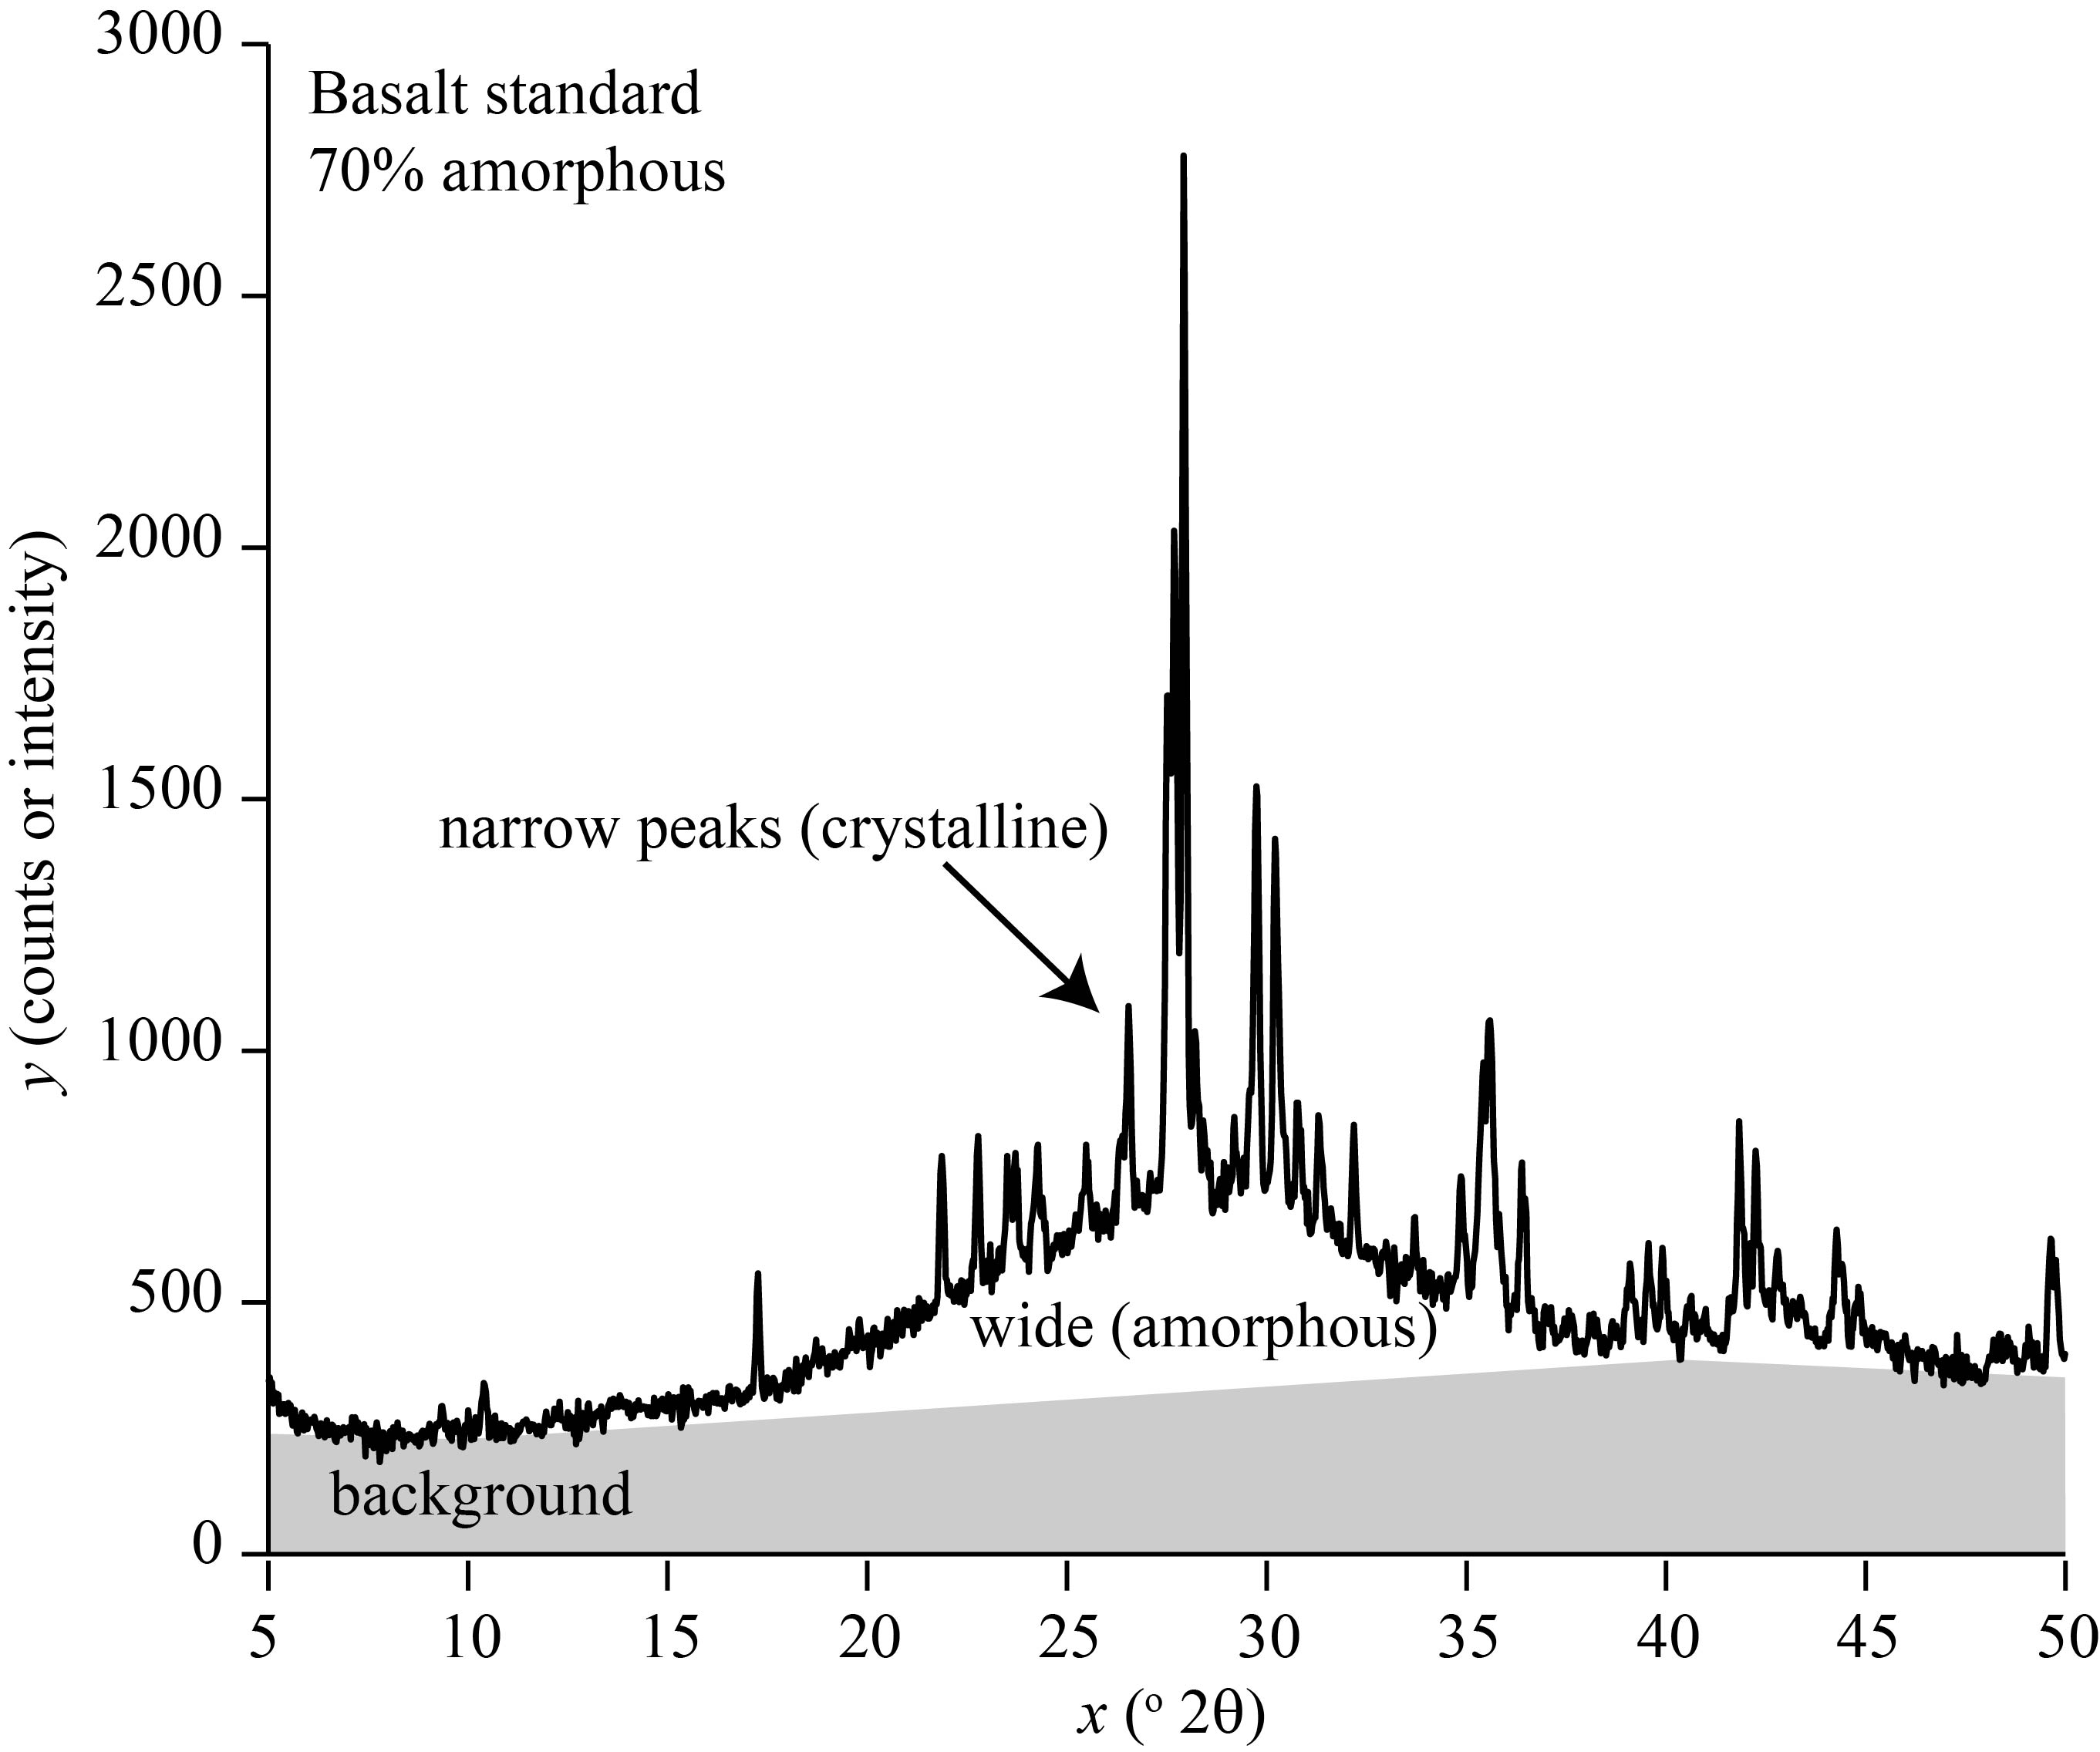
\includegraphics[width=.7\textwidth]{figures/example_data2.jpg}
\caption{\it Powder X-ray diffraction results for a basalt standard with 70\% amorphous material. Annotation corresponds to the model components: background, amorphous (wide) component, and crystalline component (narrow peaks).\label{fig:example_data2}}
\end{figure}

The model curve is a function $y = f(\x; \params)$,
which is assumed to be a sum of the following components identified in Figure~\ref{fig:example_data2}:
\begin{enumerate}
\item A background component, described by parameters $\params_{\rm bg}$
\item An amorphous component, described by parameters $\params_{\rm amorph}$
\item A crystalline component, described by parameters $\params_{\rm xtal}$
\end{enumerate}
The total model function $f_{\rm tot}(x)$ is therefore
\begin{align}
f_{\rm tot}(\x) &= f_{\rm bg}(\x; \params_{\rm bg})
       + f_{\rm amorph}(\x; \params_{\rm amorph})
       + f_{\rm xtal}(\x; \params_{\rm xtal})
\end{align}
and the measured amorphous content ($A_{\rm m}$ or $1-C_{\rm m}$) is defined, similar to Equation 1, as the proportion of the area in the
amorphous and crystalline components which is accounted for by the amorphous component:
\begin{align}
{A_{\rm m} = 1-C_{\rm m}} &= \frac{\int_{\x_{\rm min}}^{\x_{\rm max}}
            f_{\rm amorph}(\x; \params_{\rm amorph}) \, d\x}
          {\int_{\x_{\rm min}}^{\x_{\rm max}}
            f_{\rm amorph}(\x; \params_{\rm amorph}) \, dx
            + \int_{\x_{\rm min}}^{\x_{\rm max}} f_{\rm xtal}(\x; \params_{\rm xtal}) \, d\x} \label{eqn:crystallinity}
\end{align}

From each sample from the posterior distribution for all of the parameters,
it is possible to compute the proportion of amorphous material, making it straightforward to
calculate the marginal posterior distribution of the amorphous content, describing
the remaining uncertainty about its value in the light of the data.
In the following subsections, we describe the specific parameterizations of the
three parts of the model curve, that is, the functional forms of
$f_{\rm bg}$, $f_{\rm amorph}$, and $f_{\rm xtal}$.

\subsection{The background component}
The background component is assumed to be piecewise linear, with constant
slope
{between $\x=\x_{\rm min}$ and $\x=10$\degree, between $\x=10$\degree~and $\x=40$\degree,
and between $\x=40$\degree~and $\x=\x_{\rm max}$}. These values are selected to maintain a linear background over the interval from 10--40\degree, the predominant range of amorphous materials analyzed using a Cu K$\alpha$ x-ray source, while still allowing for some flexibility in the structure of the background outside this range.

We parameterized the background component using
five parameters. Firstly, there is a mean level $b$, which sets the
typical amplitude of the background component. There are also four parameters
$n_1, ..., n_4$, which determine the offset of four `control points'
from the mean level. The positions of the four control points are then:
\begin{align}
\left(\x_{\rm min}, be^{n_1}\right) \nonumber\\
\left(10, be^{n_2}\right) \nonumber\\
\left(40, be^{n_3}\right) \nonumber\\
\left(\x_{\rm max}, be^{n_4}\right). \nonumber
\end{align}
The value of the background component at any other point is found by
linear interpolation of these control points.
Figure~\ref{fig:background} shows three example
background curves generated from this parameterization, with typical
values of the parameters.

\begin{figure}[!ht]
\centering
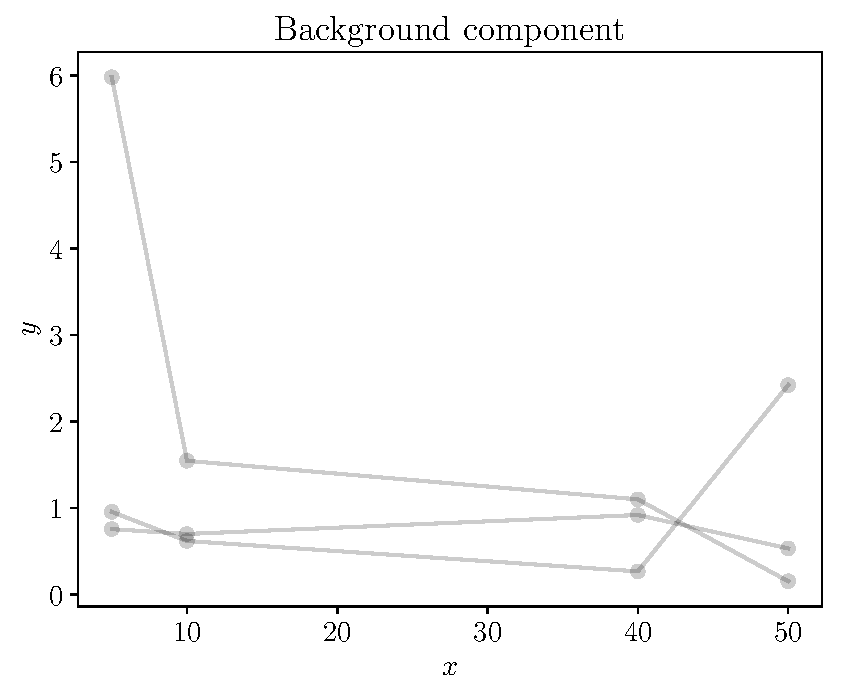
\includegraphics[width=0.6\textwidth]{figures/background.pdf}
\caption{\it Three example functions showing possible shapes of the
background component.\label{fig:background}}
\end{figure}

\subsection{The crystalline component}
We assume that there is some number $N_{\rm xtal}$ of narrow peaks,
each of which has a gaussian shape. The $i$th peak is parameterized
by its central position $X_{i, \rm xtal}$,
amplitude $A_{i, \rm xtal}$, and width $W_{i, \rm xtal}$.
The parameter vector for crystalline component is
\begin{align}
\params_{\rm xtal} &=
  \{N_{\rm xtal}, X_1, X_2, ..., X_{N, \rm xtal},
    A_1, A_2, ..., A_{N, \rm xtal},
    W_1, W_2, ..., W_{N, \rm xtal}\}
\end{align}
and the total shape contributed by the
crystalline component is a sum of the $N_{\rm xtal}$ gaussians:
\begin{align}
f_{\rm xtal}(\x; \params_{\rm xtal}) &=
    \sum_{i=1}^{N_{\rm xtal}} A_{i, \rm xtal}
 \exp\left[-\frac{1}{2W_{i, \rm xtal}^2}\left(x - X_{i, \rm xtal}\right)^2\right].
\end{align}

\subsection{The amorphous component}
The amorphous component is also composed of gaussians, like the crystalline component.
In fact, the only real difference is the prior distributions for the positions,
amplitudes, and widths, given in Section~\ref{sec:priors}.

There is some number $N_{\rm amorph}$ of gaussians in the amorphous component.
The $i$th gaussian is parameterized
by its central position $X_{i, \rm amorph}$,
amplitude $A_{i, \rm amorph}$, and width $W_{i, \rm amorph}$.
The parameter vector for wide gaussians is
\begin{align}
\params_{\rm amorph} &=
  \{N_{\rm amorph}, X_1, X_2, ..., X_{N, \rm amorph},
    A_1, A_2, ..., A_{N, \rm amorph},
    W_1, W_2, ..., W_{N, \rm amorph}\}
\end{align}
and the total shape contributed by the
amorphous component is a sum of the $N_{\rm amorph}$ gaussians:
\begin{align}
f_{\rm amorph}(\x; \params_{\rm amorph}) &=
    \sum_{i=1}^{N_{\rm amorph}} A_{i, \rm amorph}
 \exp\left[-\frac{1}{2W_{i, \rm amorph}^2}\left(x - X_{i, \rm amorph}\right)^2\right].
\end{align}

Figure~\ref{fig:wide_component} shows several examples of plausible amorphous component shapes. The prior distributions (specified in
Section~\ref{sec:priors})
constrain the central positions of these gaussians much
more strongly than the central positions of the narrow peaks (crystalline component), which is how AMORPH is able to distinguish the crystalline
component from the amorphous component.

\begin{figure}[!ht]
\centering
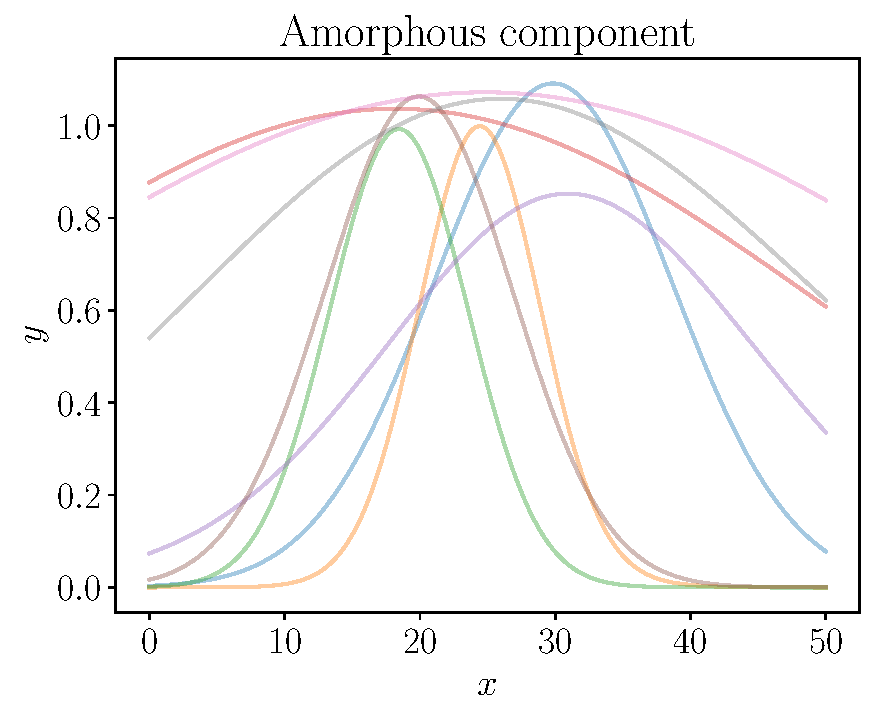
\includegraphics[scale=0.7]{figures/wide_component.pdf}
\caption{\it Some examples of plausible shapes for the amorphous component,
generated from the prior distribution for its parameters
(Section~\ref{sec:priors}). For visual purposes only, these
were scaled to amplitudes $\sim$ 1. \label{fig:wide_component}}
\end{figure}

\subsection{Derived properties}
Some derived properties of the amorphous component are used to summarize its shape.
We have included `skewness', which describes asymmetry, and `nongaussianity'
which quantifies the departure from gaussianity. These are not the same
concept, as the amorphous component could be non-gaussian while still being symmetric
(and thus having zero skewness).

Defining the normalized version of the amorphous component as
\begin{align}
g(\x) &= \frac{f_{\rm amorph}(\x)}
             {\int_{-\infty}^\infty f_{\rm amorph}(\x') \, d\x'},
\end{align}
its center of mass by
\begin{align}
\textnormal{center} &= \int_{-\infty}^\infty x g(\x) \, d\x,
\end{align}
and its width (second central moment, perhaps better interpreted
as a half-width) by
\begin{align}
\textnormal{width} &= \sqrt{\int_{-\infty}^\infty
                            g(\x) \left(\x - \textnormal{center}\right)^2
                            \, d\x},
\end{align}
the skewness is
\begin{align}
\textnormal{skewness} &= \int_{-\infty}^\infty
                           g(\x) 
                           \left(
                             \frac{x - \textnormal{center}}{\textnormal{width}}
                           \right)^3
                         \, d\x.
\end{align}

To quantify the non-gaussianity, we construct a gaussian
$g'(\x)$
with the same centre, width, and total integral as $g(\x)$, and compute the
Kullback-Leibler divergence from $g'$ to $g$:
\begin{align}
\textnormal{non-gaussianity} &= 
    \int_{-\infty}^\infty g(\x) \log\left[\frac{g(\x)}{g'(\x)}\right] \, d\x.
\end{align}
where
\begin{align}
g'(\x) &= \frac{1}{\textnormal{width} \times \sqrt{2\pi}}
            \exp\left[-\frac{1}{2\times (\textnormal{width})^2}
                    \left(\x - \textnormal{center}\right)^2\right].
\end{align}
The Kullback-Leibler divergence is a standard way of quantifying how
different one `measure' ($\equiv$ density function, for our purposes here) is from another \citep{knuth2012foundations}.
It is zero when the two measures are the same, in our case,
if $g(\x)$ is a gaussian. See Figures~\ref{fig:skewness} and~\ref{fig:nongaussianity} for example
shapes for the amorphous component, and corresponding values of the skewness
and nongaussianity.

\begin{figure}[!ht]
\centering
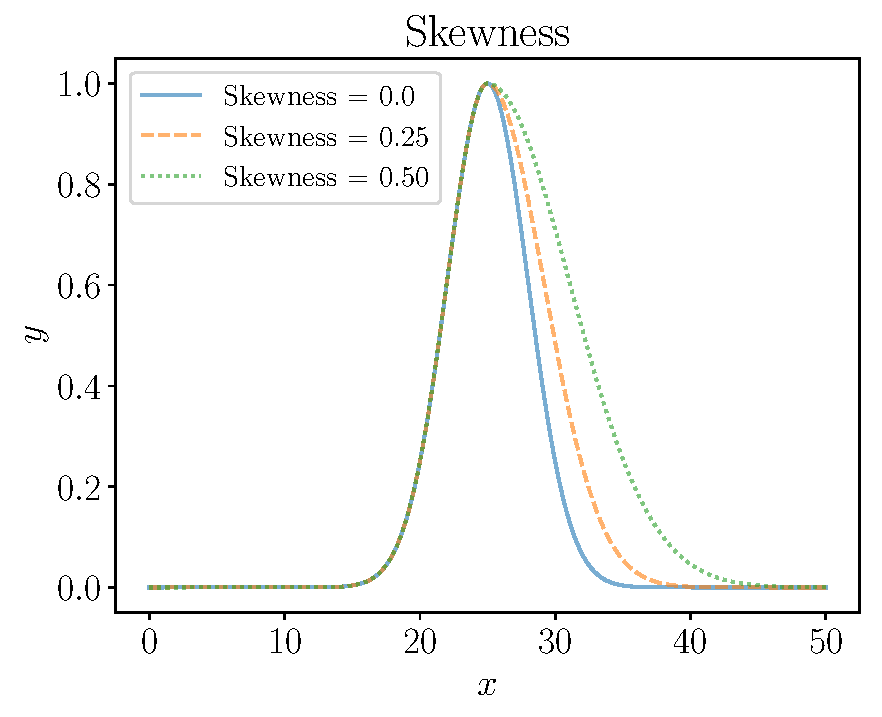
\includegraphics[width=0.6\textwidth]{figures/skewness.pdf}
\caption{\it Examples of amorphous component shapes with different values
for the skewness.\label{fig:skewness}}
\end{figure}

\begin{figure}[!ht]
\centering
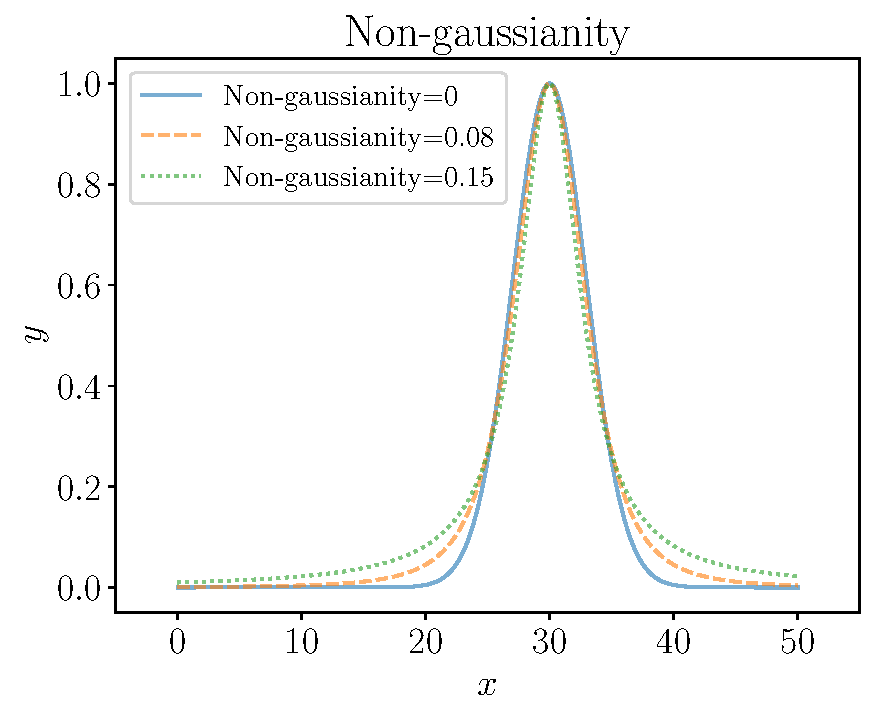
\includegraphics[width=0.6\textwidth]{figures/nongaussianity.pdf}
\caption{\it Examples of amorphous component shapes with different values
for the nongaussianity.\label{fig:nongaussianity}}
\end{figure}

\section{Prior probability distributions}\label{sec:priors}
The joint prior distribution for all of the unknown parameters and
the data must be specified.
When the number of parameters is large, this is often done `hierarchically', by
specifying the priors conditional on some `hyperparameters', and then assigning
priors to the hyperparameters.

The joint prior distribution for
the hyperparameters, parameters, and data,
is written $p(\hypers, \params, \data | \info)$, and is usually factorized
in this way:
\begin{align}
p(\hypers, \params, \data | \info) &=
    p(\hypers | \info)p(\params | \hypers, \info)
    p(\data | \params, \hypers, \info)\\
    &= p(\hypers | \info)p(\params | \hypers, \info)
    p(\data | \params, \info)
\end{align}
where the first step is true in general by the product rule, and the second
step assumes that knowing the parameters would make the hyperparameters
irrelevant when predicting what data would be observed. In the AMORPH model,
we introduced hyperparameters describing the typical amplitude
and width of the gaussians for the amorphous component, and
the degree to which the actual amplitudes and widths are scattered
around that typical value. This was also done for the crystalline
component.

A directed acyclic graph, also known as a probabilistic graphical model (PGM),
which depicts the dependence structure of the entire joint
prior probability distribution,
is shown in Figure~\ref{fig:pgm-edited}. The prior distributions themselves
are specified in Table~\ref{tab:priors}.

\begin{figure}[!ht]
\centering
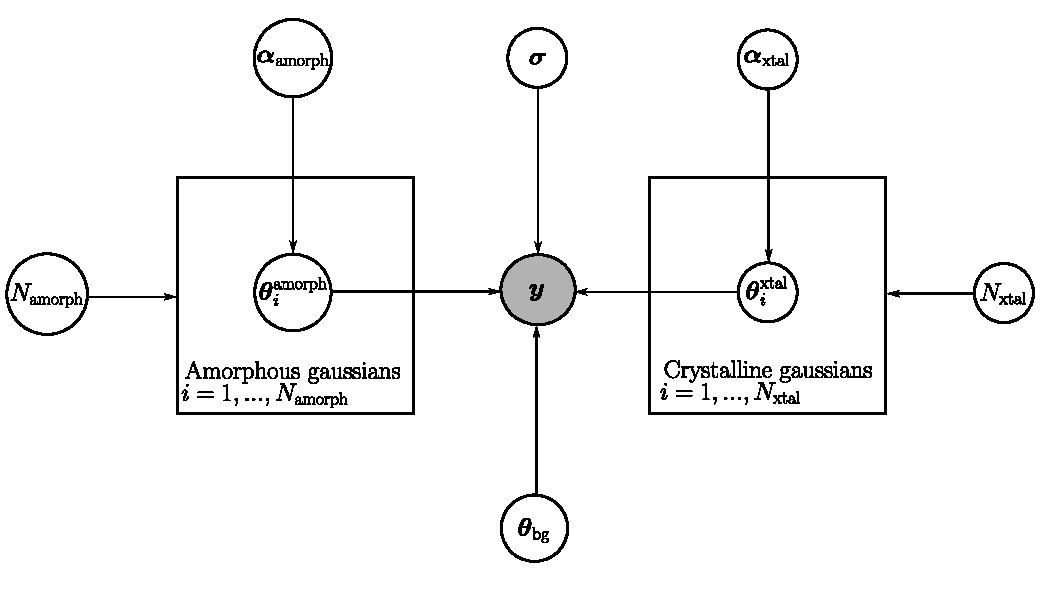
\includegraphics[scale=0.7]{figures/pgm-edited.pdf}
\caption{The PGM. The hyperparameters controlling the prior distributions
for the amorphous and crystalline gaussians are denoted collectively
by $\boldsymbol{\alpha}_{\rm amorph}$ and
$\boldsymbol{\alpha}_{\rm xtal}$ respectively.
The noise-related parameters are collected under $\boldsymbol{\sigma}$.
The data is $\boldsymbol{y}$.\label{fig:pgm-edited}}
\end{figure}

\begin{landscape}

\begin{table}
\footnotesize
\centering
\begin{tabular}{|lll|}
\hline
{\bf Quantity}      &   {\bf Meaning}   &  {\bf Prior distribution}\\
\hline
{\em Prior information}&&\\
\hline
$n$ & Number of measurements & given\\
$\{\x_1, \x_2, ..., \x_n\}$  & $\x$-values of measurements & given \\
\hline
{\em Hyperparameters} & &\\
$N_{\rm xtal}$   &   Number of narrow peaks    &  $\propto 1/(N_{\rm xtal}+1)$, $N_{\rm xtal} \in \{0, 1, ..., 300\}$ \\
$N_{\rm amorph}$   &   Number of wide peaks    &  $\propto 1/(N_{\rm amorph}+1)$,
$N_{\rm amorph} \in \{0, 1, ..., 300\}$ \\
$a_{\ln A, \rm xtal}$ & Typical log-amplitude of narrow peaks & Laplace(0, 5)\\
$a_{\ln A, \rm amorph}$ & Typical log-amplitude of wide peaks & Laplace(0, 5)\\
$b_{\ln A, \rm xtal}$ & Diversity of log-amplitude of narrow peaks & Uniform(0, 5)\\
$b_{\ln A, \rm amorph}$ & Diversity of log-amplitude of wide peaks & Uniform(0, 5)\\
$a_{\ln W, \rm xtal}$ & Typical log-width of narrow peaks & LogUniform$(10^{-3}x_{\rm range}, 0.05x_{\rm range})$\\
$a_{\ln W, \rm amorph}$ & Typical log-width of wide peaks & LogUniform$(0.05x_{\rm range}, x_{\rm range})$\\
$b_{\ln W, \rm xtal}$ & Diversity of log-width of narrow peaks & Uniform(0, 0.1)\\
$b_{\ln W, \rm amorph}$ & Diversity of log-width of wide peaks & Uniform(0, 0.2)\\
\hline
{\em Background parameters}&&\\
$b$       & Mean background level       & $\ln b \sim $ Laplace$(0, 5)$\\
$\{n_1, ..., n_4\}$  & Background deviations & independent Normal$(0,1)$\\
\hline
{\em Crystalline parameters}&&\\
$X_{i, \rm xtal}$ & Positions of narrow peaks &
                            Uniform$(x_{\rm min}, x_{\rm max})$ \\
$A_{i, \rm xtal}$ & Amplitudes of narrow peaks &
 $\ln A_{i, \rm xtal} \sim \textnormal{Laplace}\left(a_{\ln A, \rm xtal}, b_{\ln A, \rm xtal}\right)$ \\
$W_{i, \rm xtal}$ & Widths of narrow peaks &
 $\ln W_{i, \rm xtal} \sim \textnormal{Laplace}\left(a_{\ln W, \rm xtal}, b_{\ln W, \rm xtal}\right)$ \\
\hline
{\em Amorphous parameters}&&\\
$X_{i, \rm amorph}$ & Positions of wide peaks &
          Uniform$(x_{\rm min}+0.3x_{\rm range}, x_{\rm max}-0.3x_{\rm range})$ \\
$A_{i, \rm amorph}$ & Amplitudes of wide peaks &
 $\ln A_{i, \rm amorph} \sim \textnormal{Laplace}\left(a_{\ln A, \rm amorph}, b_{\ln A, \rm amorph}\right)$ \\
$W_{i, \rm amorph}$ & Widths of wide peaks &
 $\ln W_{i, \rm amorph} \sim \textnormal{Laplace}\left(a_{\ln W, \rm amorph}, b_{\ln W, \rm amorph}\right)$ \\
\hline
{\em Noise parameters}&&\\
$\sigma_0$ &    Constant noise level  &   $\ln \sigma_0 \sim \textnormal{Laplace}(0,5)$\\
$\sigma_1$ &    Noise proportional to $\sqrt{\textnormal{model}}$   &  $\ln \sigma_1 \sim \textnormal{Laplace}(0,5)$ \\
$\nu$     &   Shape parameter for $t$-distribution for noise   &   LogUniform$(1, 1000)$\\
\hline
{\em Data}&&\\
\hline
$\{y_1, y_2, ..., y_n\}$  &   Measurements    & independent Student-$t(f(x_i; \params), \sqrt{\sigma_0^2 + \sigma_1f(x_i; \params)},\nu)$\\
\hline
\end{tabular}
\caption{\it The prior distributions for all hyperparameters,
parameters, and the data.\label{tab:priors}}
\end{table}

\end{landscape}

Most of the chosen distributions were intended to be reasonably
conservative and wide.
Some of the prior distributions in AMORPH use the log-uniform distribution,
sometimes (erroneously) called a Jeffreys prior, whose density for a quantity
$z$ is proportional to $1/z$.

We used a Laplace distribution for some informative priors, rather than
a more conventional normal distribution, because it assigns higher
prior probability to values far from the center, and can be computed conveniently, i.e., no special functions such as the inverse of the
error function are needed.
The Laplace, or biexponential, distribution with location parameter
(central position) $a$ and scale parameter (width) $b$ has probability
density given by
\begin{align}
p(x | a, b) &= \frac{1}{2b}\exp\left[-\frac{|x - a|}{b}\right].
\end{align}

The priors for the positions and widths of the `amorphous' and `crystalline'
gaussians are different, to account for the prior knowledge that they
should result in wide gaussians near the centre of the domain, and
narrow gaussians throughout the domain respectively.

The prior for the data given all the parameters is a student-$t$ distribution,
which allows for potentially heavier tails than a normal distribution would.
Thus, analyses with AMORPH should be able to cope with discrepant datapoints
as long as they are not locally correlated (which would cause them to be
mistaken for peaks).

AMORPH does not assume a known number of gaussians for either the
amorphous or the crystalline component. The appropriate number of
gaussians is inferred from the data. The maximum number of gaussians
in each component is set to 300.

\section{Applications}\label{sec:applications}
\subsection{Crystallinity}
The AMORPH program calculates a fraction of amorphous material ($A_{\rm m}$) for each posterior sample of the parameters,
using Equation~\ref{eqn:crystallinity}.Thus measured crystallinity ($C_{\rm m}$) is easily determined from the relationship $C_{\rm m}$ = 1-$A_{\rm m}$, as defined in Equation 5. The measured crystallinity is not equivalent to an "actual" or "true" crystallinity, although the values are often very close to one another.
It should therefore be noted that this procedure does not negate the need for calibration standards
to translate measured crystallinity to an actual crystallinity. Transmission and absorption of X-rays in the material will vary as the ratio of mineral to glass changes in the sample, causing a deviation from a 1:1 line. In addition to theoretical considerations, practical challenges also exist for background fitting. At low crystallinity ($\lesssim 10\%$) diffraction patterns are dominated by the low amplitude amorphous peak such that removing the effects of background noise becomes problematic, resulting in overestimated crystallinities. At high crystallinity ($\gtrsim 90\%$) the problem arises that peak overlaps in multi-mineral assemblages cause broadening effects, and may be subsequently modeled as ``amorphous'' and thus crystallinities  underestimated. The calibration curve therefore is utilized to remove these effects. This is also an important step as
different X-ray diffractometers will provide slightly different calibration curves (Fig.~\ref{fig:intruments}).
Differences between instruments largely reflect changes in background intensity and shape,
particularly at low values of $2\theta$. 

	Calibration standards can be easily created by mixing
powdered minerals (e.g. olivine, pyroxene, plagioclase) with powdered glass in known
proportions to simulate volcanic material of varying crystallinities \citep[e.g.,][]{rowe2012, wall2014}.
Results of the AMORPH calculations show good agreement to calibration curves using the manual
calibration approach (Fig.~\ref{fig:Comparison}). The offset between the AMORPH and manual calibration methods
in Figure~\ref{fig:Comparison} is consistent with the change in analyzed $2\theta$ range, 10--40\degree~and 5--50\degree,
respectively (Fig.~\ref{fig:Outputs}). Since the wide peak for the amorphous material does not extend
appreciably out of the range from 10--40\degree~$2\theta$ (for a Cu K$\alpha$ source), peak integration
outside of this range will decrease the relative contribution of the amorphous material
(only peaks for crystalline materials are outside this range). Experimentation demonstrates also that data processing only over the 10--40\degree~$2\theta$ range is also significantly faster, as this reduces the total number of data points for processing. Thus we recommend that the optimal range for data processing in terms of time and accuracy is from 10--40\degree~$2\theta$.


\begin{figure}[!ht]
\centering
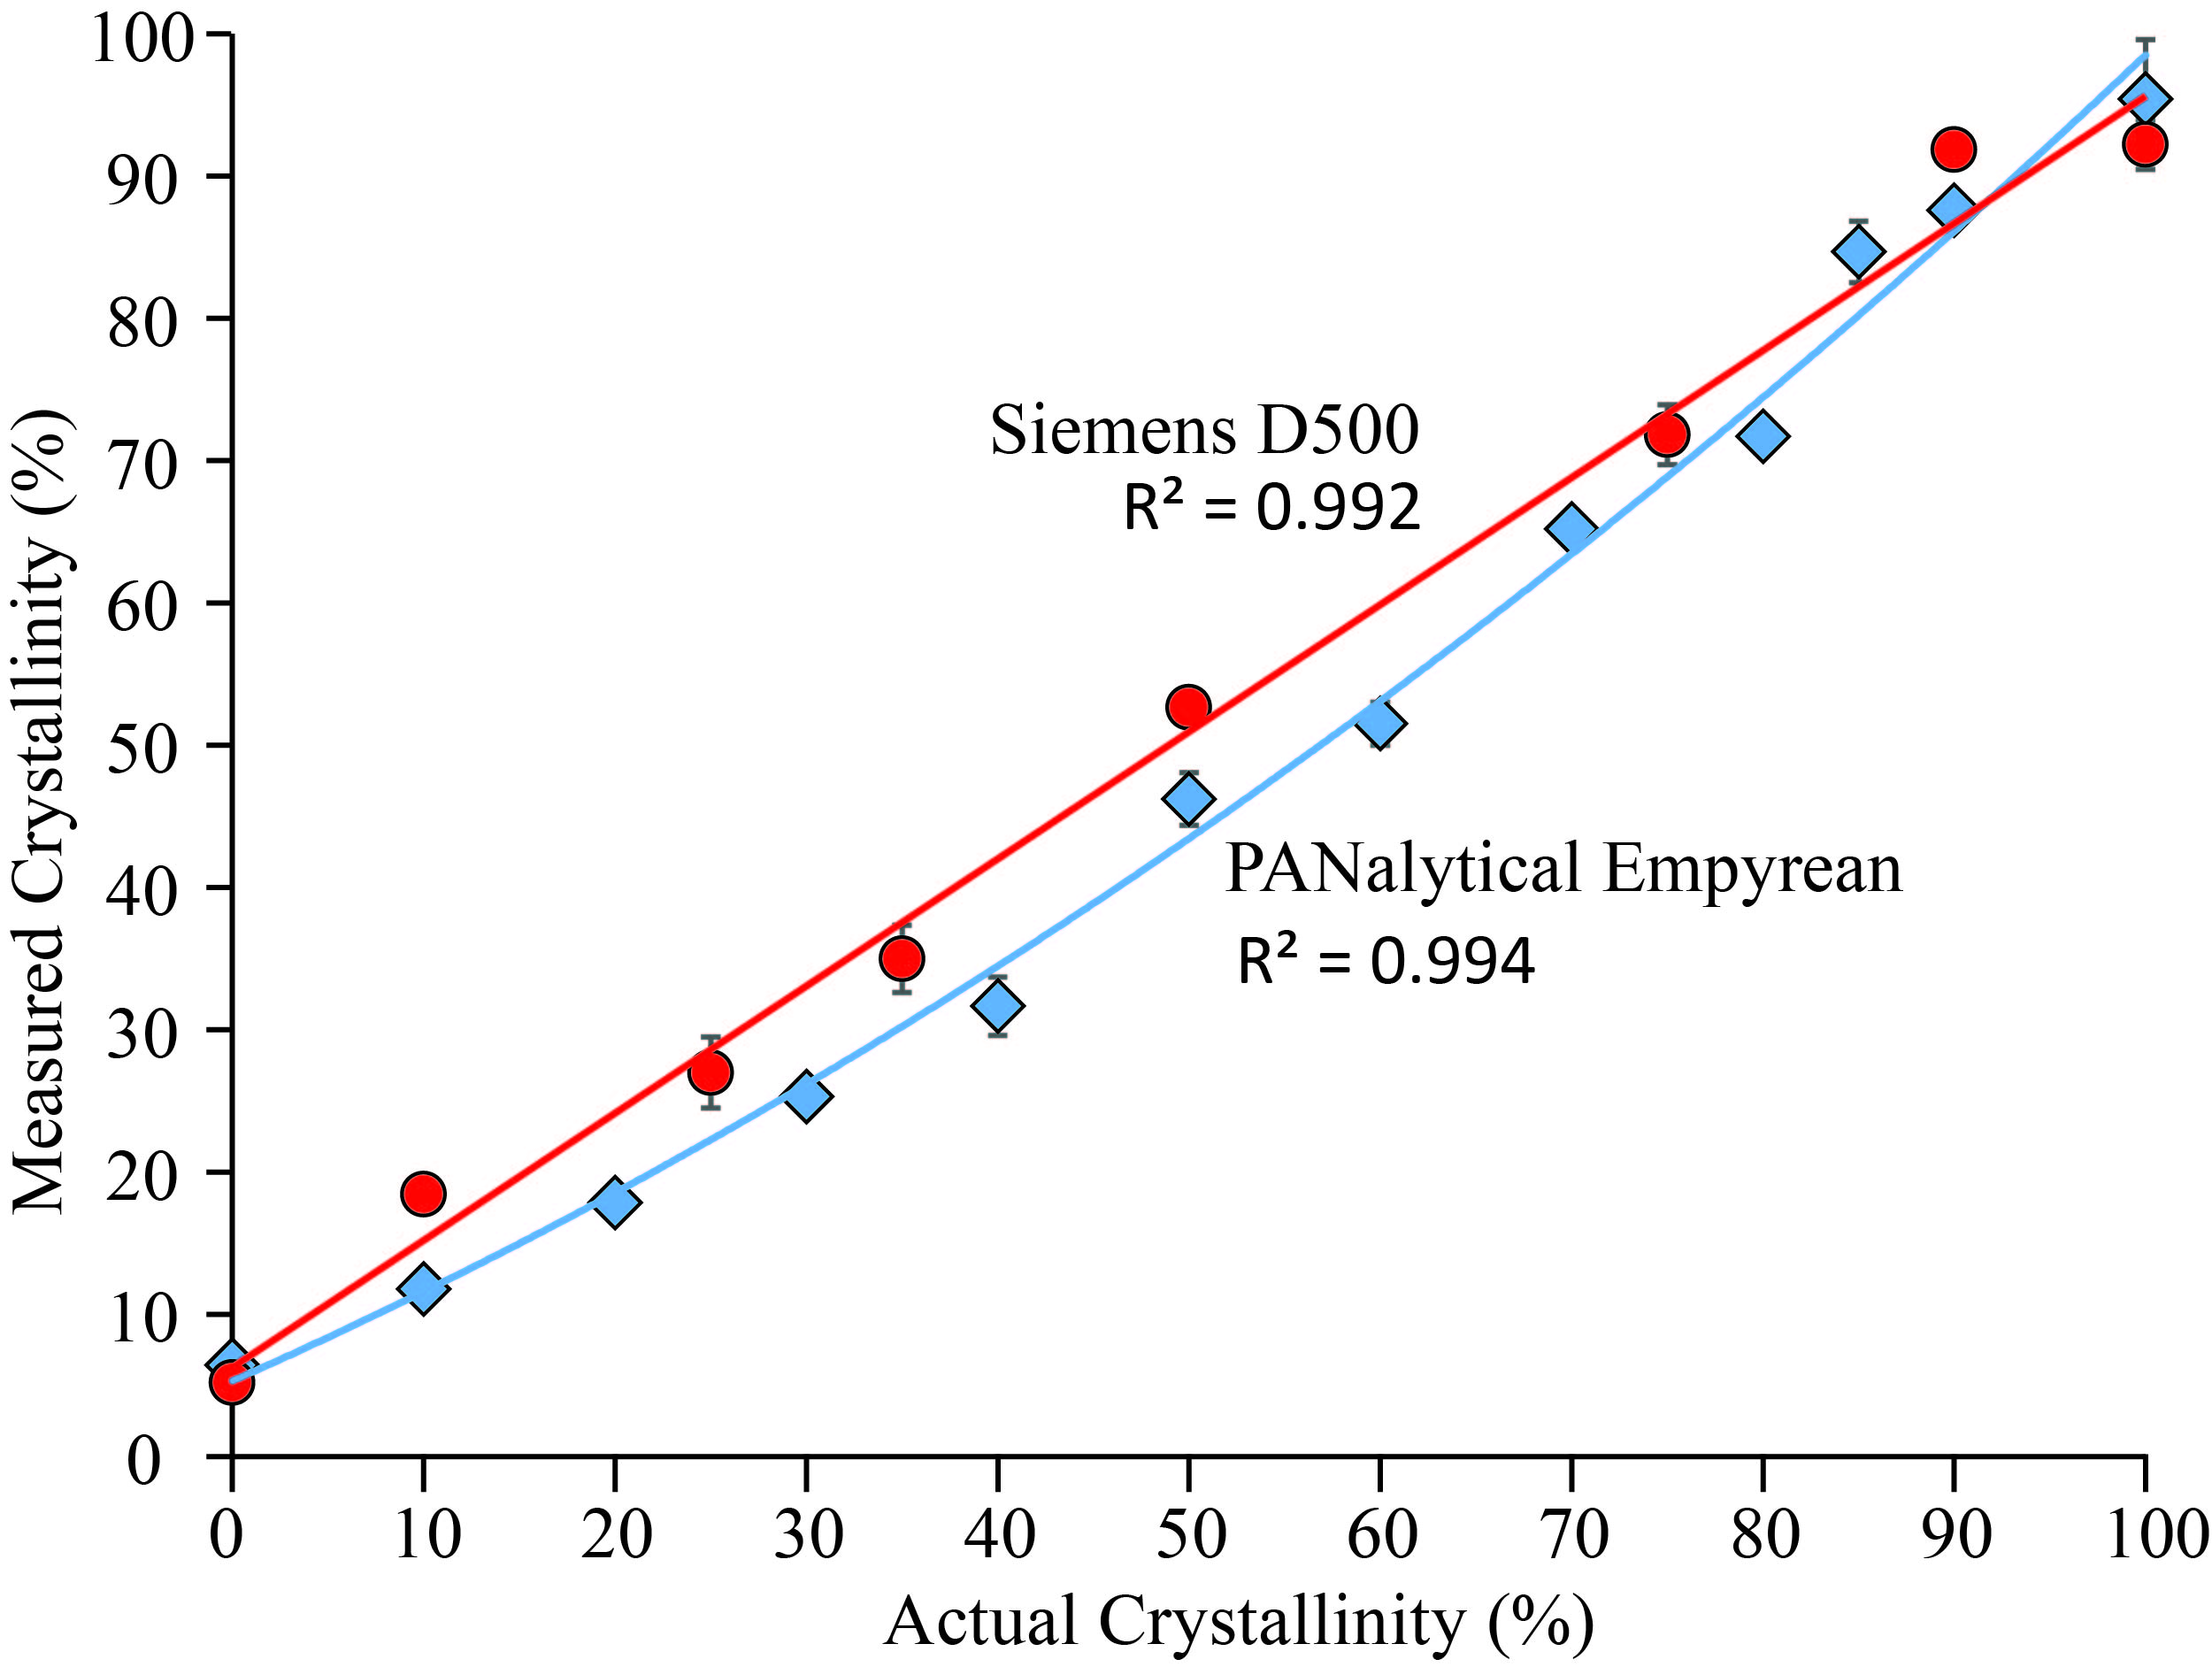
\includegraphics[width=0.7\textwidth]{figures/instruments.jpg}
\caption{\it Two calibration curves of the same standard material (rhyolite) are compared from different instrumentation, including a Siemens D500 (Washington State University; red circles) and a PANalytical Empyrean (University of Auckland; blue diamonds).\label{fig:intruments}}
\end{figure}

\begin{figure}[!ht]
\centering
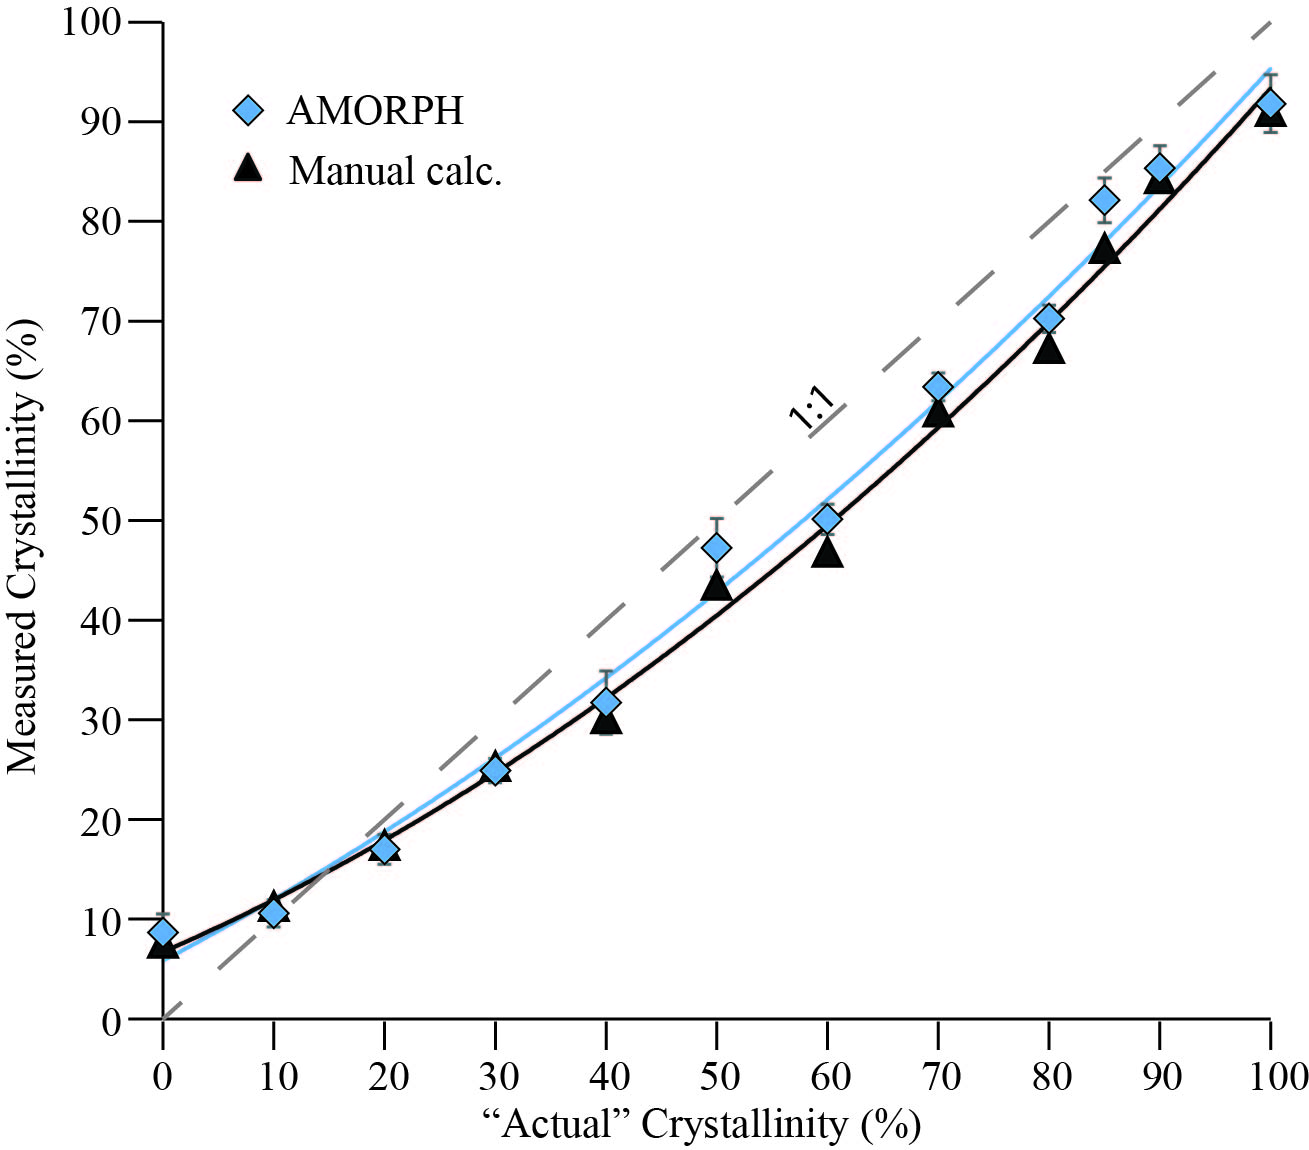
\includegraphics[width=0.7\textwidth]{figures/Comparison.jpg}
\caption{\it Comparison of calibration results for rhyolite calculated from AMORPH compared to a calibration calculated using the manual procedure described by \citet{rowe2012}.\label{fig:Comparison}}
\end{figure}

\begin{figure}[!ht]
\centering
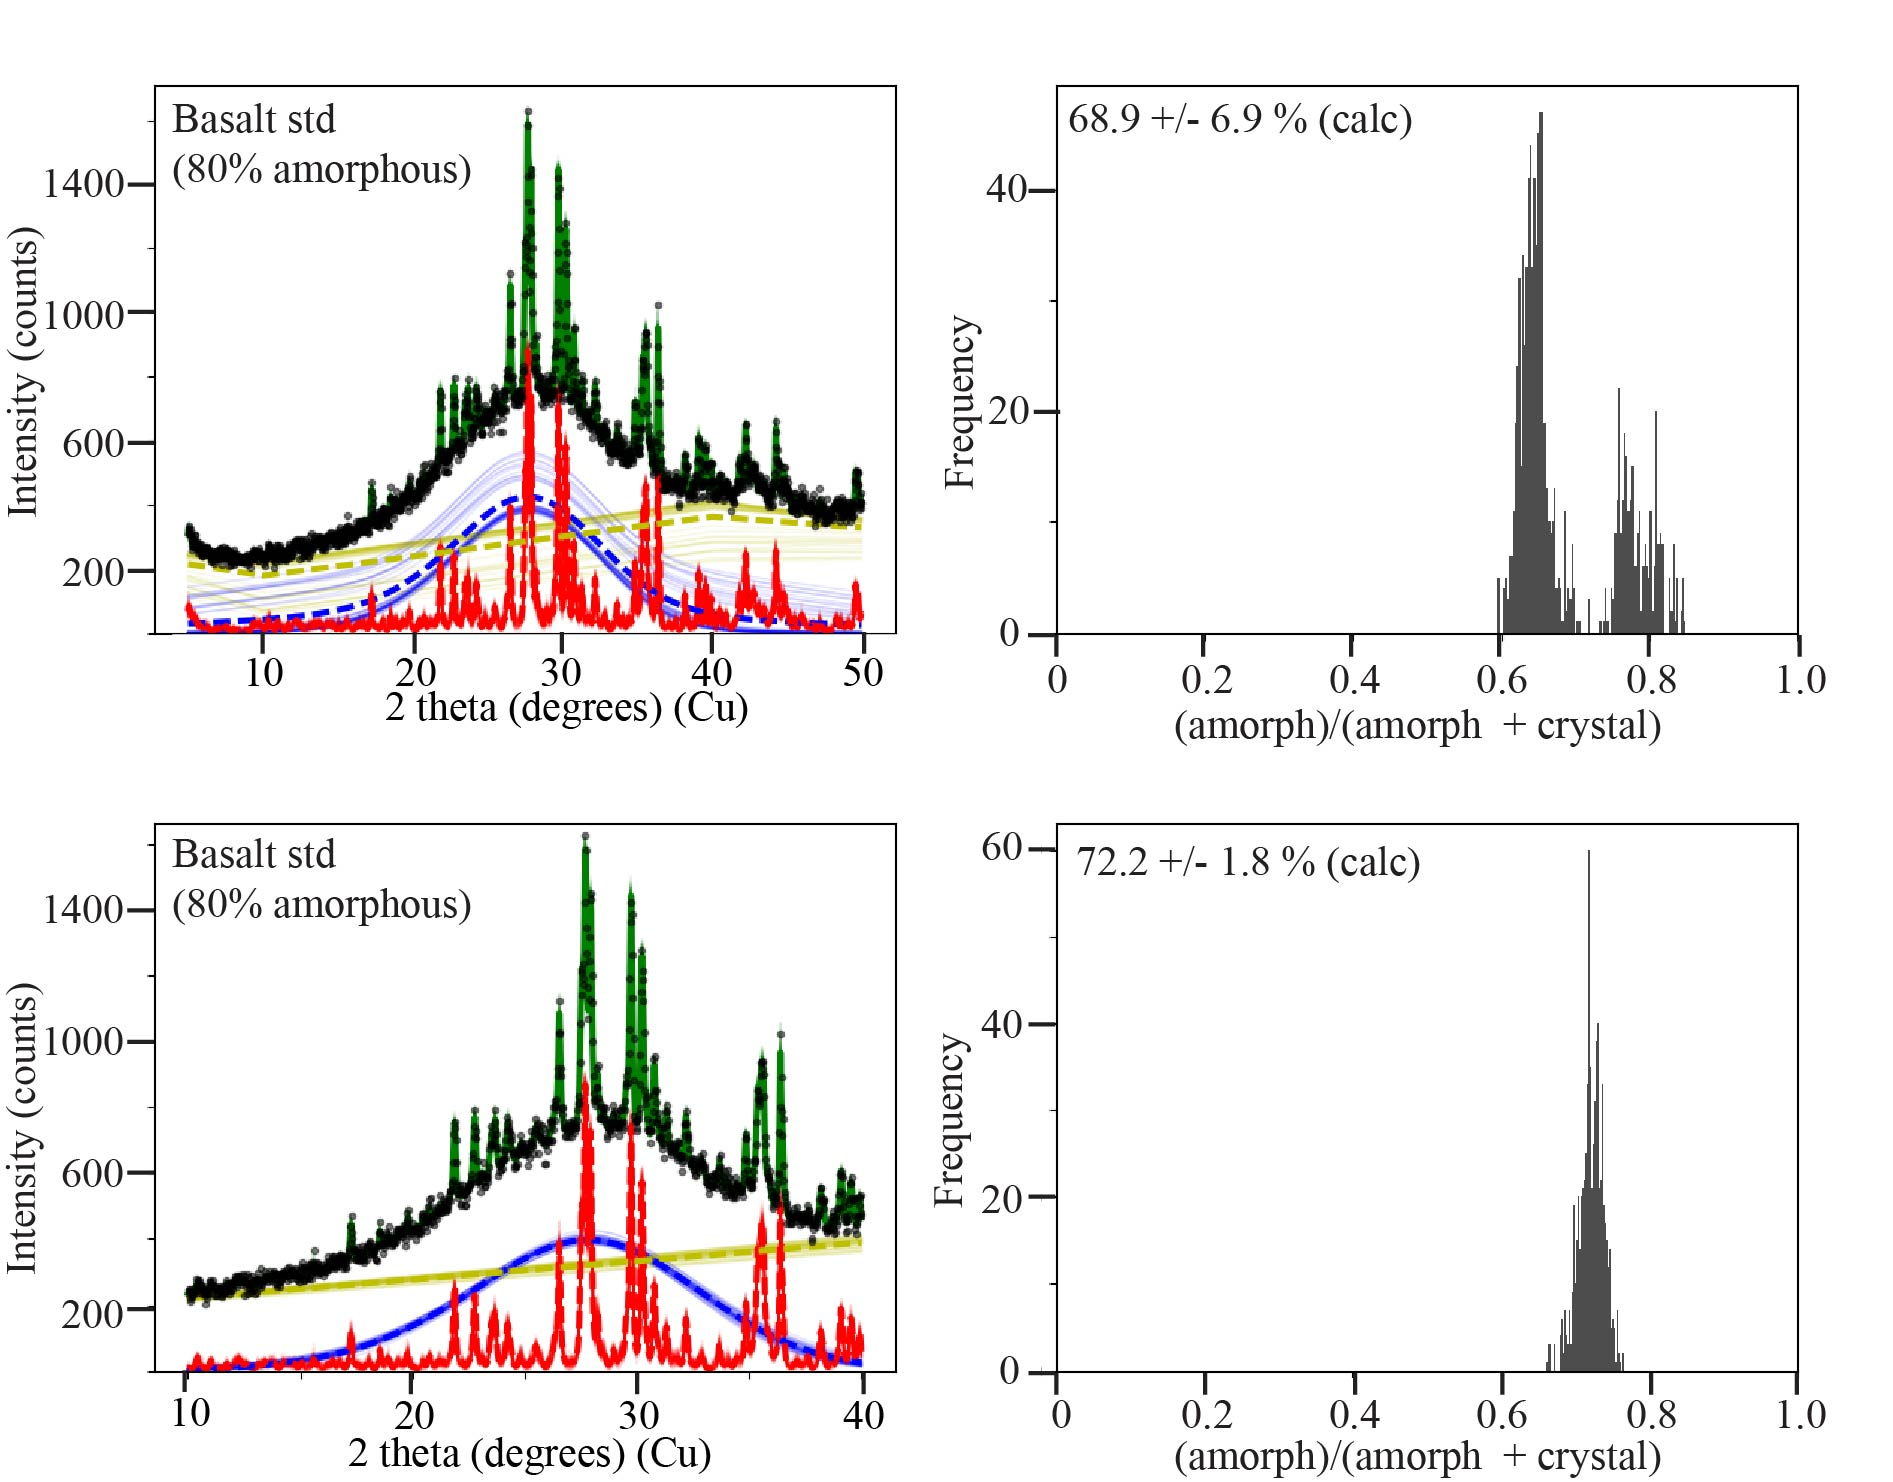
\includegraphics[width=1\textwidth]{figures/Outputs.jpg}
\caption{\it Model results for a basalt standard containing 80\% amorphous glass. Data was processed from 10--40\degree~$2\theta$ (upper left panel) with a calculated amorphous content of 76.4\% (upper right panel). The same data was processed instead from 5--50\degree~$2\theta$ (lower left panel) with a calculated amorphous content of 71.5\% (lower right panel). Rationale for differences are discussed in the text.\label{fig:Outputs}}
\end{figure}

\subsection{Amorphous Characteristics}
As discussed above, one of the primary advantages of the AMORPH program is that it can
independently model characteristics of the amorphous component.  In particular, centre of mass,
skewness, and nongaussianity are distinctive amongst different amorphous materials. To test
this, we present amorphous characteristics of rhyolite and basalt glass picked from a
Taupo pumice \citep[73.5 wt\% SiO\textsubscript{2}; P2166C;][]{barker2015} and a Kilauea basalt
\citep[51 wt\% SiO\textsubscript{2}; KS08-108E;][]{wooten2009, rowe2015}, respectively.
In addition, Mars Scientific Laboratory (MSL) Curiosity rover CheMin instrument reduced X-ray diffraction patterns
for sediments from the Bagnold Sand Dunes \citep[Gobabeb;][]{achilles2017, lapotre2017}
and Buckskin \citep{morris2016} localities, both which have significant amorphous
materials, have been processed for comparison (CheMin instrument data\footnote{\tt http://pds-geosciences.wustle.edu/missions/msl/chmin.htm}). MSL diffraction patterns have been
recalculated from a Co K$\alpha$ ($1.7890 \dot{A}$) to Cu K$\alpha$ ($1.5406 \dot{A}$) X-ray source using Bragg's law, to be visually comparable to terrestrial
examples analysed for this study. Results are summarized in Figure~\ref{fig:volcanic_glasses}. The most notable differences in the amorphous component characteristics calculated for diffraction patterns for basalt and rhyolite glass include a positive skewness and shift to lower centre of mass
$2\theta$ values for the rhyolite glass compared to the basalt glass. Although, CheMin
diffraction analyses were run on a different X-ray diffractometer from the terrestrial
samples shown here, similar relative changes in amorphous characteristics can be observed
in X-ray diffraction data from Mars. In particular, the Buckskin 1 analysis of the amorphous component indicates a positive skewness $\sim 4\times$ greater than in the Gobabeb 2 sample. These results suggest a distinct change in the
composition of the amorphous material. This interpretation, is consistent with prior
published results which suggest that at the Gobabeb locality (Namib Dune, Bagnold Dune Field),
the sample is dominated by a basaltic mineralogy, while at the Buckskin locality,
the amorphous component has been calculated to contain ~77 wt\% SiO\textsubscript{2}
\citep[i.e. rhyolitic;][]{morris2016, achilles2017}. 

\begin{figure}[!ht]
\centering
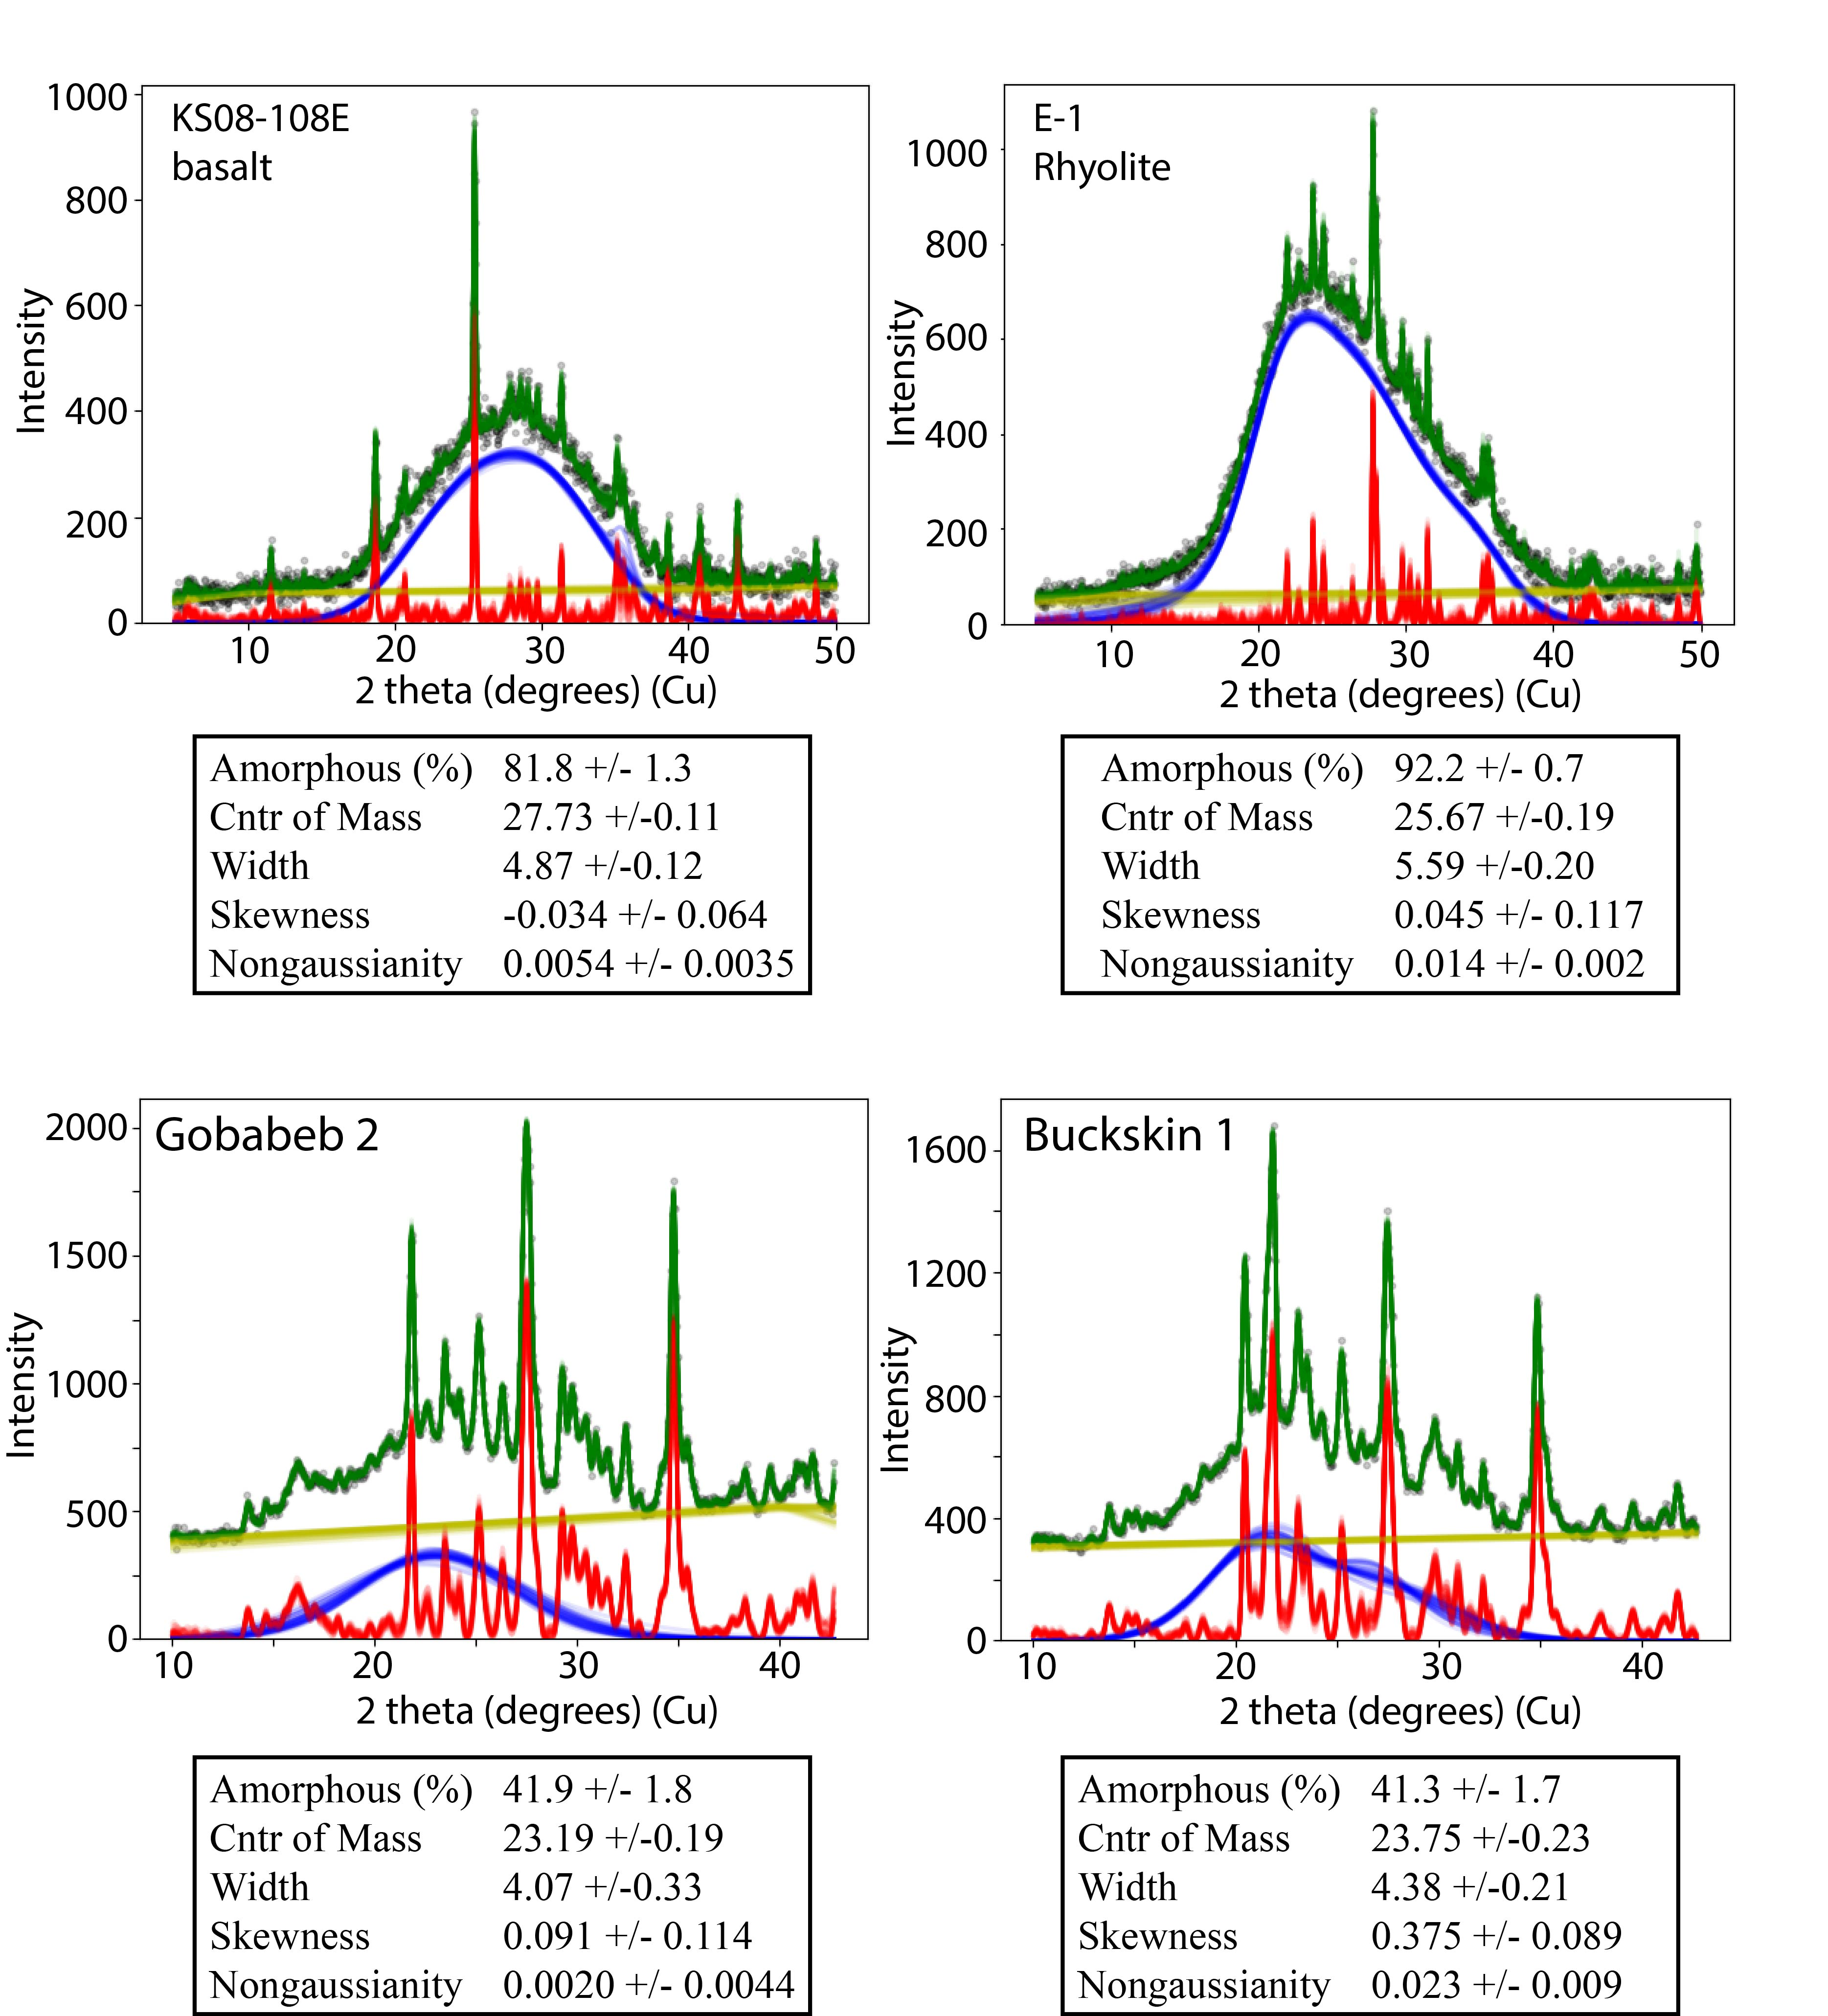
\includegraphics[width=1\textwidth]{figures/volcanic_glasses.jpg}
\caption{\it Four examples of changing characteristics of amorphous material based on composition. Kilauea basalt glass (upper left) and taupo rhyolite glass (upper right) were analyzed on a PANalytical Empyrean XRD at University of Auckland. Gobabeb 2 (lower left) and Buckskin 1 (lower right) results from the CheMin instrument on the MSL Curiosity rover (data sourced as above). Calculated statistics for each analysis are provided below the model results. Note in particular the change in skewness from Basalt to Rhyolite, and from Gobabeb 2 to Buckskin 1, supporting compositional change.\label{fig:volcanic_glasses}}
\end{figure}

\section{Conclusions}\label{sec:conclusions}
The AMORPH program’s statistical approach to interpreting amorphous materials in X-ray
diffraction patterns provides a new and unique methodology.
By explicitly specifying a set of assumptions and computing their
implications, we can automatically produce outputs separating the
amorphous and crystalline components and quantifying their properties,
along with a corresponding uncertainty estimate for any inferred
quantity.
A significant outcome of this research is that it reduces intra- and inter-user variability
by eliminating the need for manual background fitting, the largest source of error in the
calibration methodology for quantifying the amorphous component. Results demonstrate that
this approach 1) accurately reproduces values of known crystallinity and 2) is consistent
with prior manual approaches to the calibration method. Quantification of the amorphous
content however still requires a calibration curve to correct for x-ray absorption/emission
in heterogeneous materials, and to remove systematic biases in both background fitting and instrumentation. 

In addition to the quantification of amorphous and crystalline components, the AMORPH
program calculates statistical parameters of the amorphous component, including the centre
of mass, width of amorphous component, skewness, and nongaussianity. Characterization of the amorphous component requires no calibration and outputs show 
clear distinctions, in particular in terms of skewness, as a function of changing composition of the amorphous material in the demonstrated examples of
geologic materials from Earth and Mars.


\section*{Acknowledgments}

BJB was supported by a Marsden Fast-Start grant from the Royal Society of
New Zealand from 2013 to 2016, and this work is a spinoff from that
project. Data used in Figure~\ref{fig:volcanic_glasses} analyzed and processed by J. Li, M. Jugo, A. Serrano. Manual calibration for Figure~\ref{fig:Comparison} was conducted by Y. Heled. This project made use of the resources of the Centre for
eResearch at the University of Auckland.

\section*{References}
\begin{thebibliography}{99}
\bibliographystyle{plainnat}

\bibitem[Achilles et al.(2017)]{achilles2017}
Achilles, C.N., et al. 2017. Mineralogy of an active eolian sediment from the Namib Dune, Gale Crater, Mars. Journal of Geophysical Research Planets, doi: 10.1002/2017JE005262.

\bibitem[Achilles et al.(2013)]{achilles2013}
Achilles, C.N., Morris, R.V., Chipera, S.J., Ming, D.W., Rampe, E.B. 2013. X-ray diffraction reference intensity ratios of amorphous and poorly crystalline phases: Implications for CheMin on the Mars Science Laboratory mission. 44th Lunar and Planetary Science Conference.

\bibitem[Barker et al.(2015)]{barker2015}
Barker, S.J., Wilson, C.J.N., Allan, A.S.R., Schipper, C.I. 2015. Fine-scale temporal recovery, reconstruction and evolution of a post-supereruption magmatic system. Contributions to Mineralogy and Petrology, 170:5; doi: 10.1007/s00410-015-1155-2.

\bibitem[Berger et al.(2016)]{berger2016}
Berger, J.A., et al. 2016. A global Mars dust composition refined by the Alpha-Particle X-ray Spectrometer in Gale Crater. Geophysical Research Letters, 43, 67-75.

\bibitem[Bish et al.(2013)]{bish2013}
Bish, D. L. et al. 2013. X-ray diffraction results from Mars Science Laboratory: mineralogy of Rocknest at Gale Crater. Science, 341, 1238932.

\bibitem[Blake et al.(2013)]{blake2013}
Blake, D. F. et al. 2013. Curiosity at Gale Crater, Mars: characterization and analysis of the Rocknest sand shadow. Science, 341, 1239505.

\bibitem[Brewer et al.(2011)]{dns}
Brewer, B. J., Pártay, L. B., \& Csányi, G. (2011). Diffusive nested sampling. Statistics and Computing, 21(4), 649-656.

\bibitem[{Brewer} and {Foreman-Mackey}(2016)]{dnest4}
Brewer, B. J., Foreman-Mackey, D.
\newblock {DNest4: Diffusive Nested Sampling in C++ and Python}.
\newblock \emph{Journal of Statistical Software, accepted. arxiv: 1606.03757},
  June 2016.

\bibitem[Chipera and Bish(2002)]{chipera2002}
Chipera, S.J., Bish, D.L. 2002. FULLPAT: a full-pattern quantitative analysis program for X-ray powder diffraction using measured and calculated patterns. Journal of Applied Crystallography, 35, 744-749.

\bibitem[Dehouck et al.(2014)]{dehouck2014}
Dehouck, E., McLennan, S.M., Meslin, P-Y., Cousin, A. 2014. Constraints on abundance, composition and nature of X-ray amorphous components of soils and rocks at Gale crater, Mars. Journal of Geophysical Research Planets, 119, 2640-2657.

\bibitem[Ellis et al.(2015)]{ellis2015}
Ellis, B.S., Cordonnier, B., Rowe, M.C., Szymanowski, D., Bachmann, O., Andrews, G.D.M. 2015. Groundmass crystallisation and cooling rates of lava-like ignimbrites: the Grey’s Landing ignimbrite, southern Idaho, USA. Bulletin of Volcanology, doi 10.1007/s00445-015-0972-5.

\bibitem[Gregory(2005)]{gregory2005bayesian}
Gregory, P. C.
\newblock \emph{Bayesian Logical Data Analysis for the Physical Sciences: A
  Comparative Approach with Mathematica{\textregistered} Support}.
\newblock Cambridge University Press, 2005.

\bibitem[Gualtieri(1996)]{gualtieri1996}
Gualtieri, A. 1996. Modal analysis of pyroclastic rocks by combined Rietveld and RIR methods. Powder Diffraction, 11(2), 97-106.

\bibitem[Gualtieri(2000)]{gualtieri2000}
Gualtieri, A. 2000. Accuracy of XRPD QPA using the combined Rietveld-RIR method. Journal of Applied Crystallography, 33, 267-278.

\bibitem[Kanakiya et al.(2017)]{kanakiya2017}
Kanakiya, S., Adam, L., Esteban, L., Rowe, M.C., Shane, P. 2017. Dissolution and secondary mineral precipitation in basalts due to reactions with carbonic acid, Journal of Geophysical Research Solid Earth, 122, 4312-4327, doi:10.1002/2017JB014019.

\bibitem[Knuth and Skilling(2012)]{knuth2012foundations}
Knuth, K. H., Skilling, J.
\newblock Foundations of inference.
\newblock \emph{Axioms}, 1\penalty0 (1):\penalty0 38--73, 2012.

\bibitem[Lapotre et al.(2017)]{lapotre2017}
Lapotre, M.G.A., Ehlmann, B.L., Minson, S.E., Arvidson, R.E., Ayoug, F., Fraeman, A.A., Ewing, R.C., Bridges, N.T. 2017. Compositional variations in sands of the Bagnold Dunes, Gale Crater, Mars, from Visible-Shortwave Infrared Spectroscopy and comparison with ground truth from the Curiosity Rover, Journal of Geophysical Research Planets; doi: 10.1002/2016JE005133.

\bibitem[Mackay(2003)]{mackay2003}
MacKay, D. J. C. (2003). Information theory, inference and learning algorithms. Cambridge university press.

\bibitem[Morris et al.(2016)]{morris2016}
Morris, R.V., et al. 2016. Silicic volcanism on Mars evidenced by tridymite in high-SiO2 sedimentary rock at Gale crater. PNAS, 113 (26), 7071-7076.

\bibitem[O'Hagan and Forster(2004)]{o2004kendall}
O'Hagan, A., Forster, J. J.
\newblock \emph{Kendall's advanced theory of statistics, volume 2B: Bayesian
  inference}, volume~2.
\newblock Arnold, 2004.

\bibitem[Rowe et al.(2012)]{rowe2012}
Rowe, M.C., Ellis, B.S., Lindeberg, A. 2012. Quantifying crystallization and devitrification of rhyolites by means of X-ray diffraction and electron microprobe analysis. American Mineralogist, 97, 1685-1699.


\bibitem[Rowe et al.(2015)]{rowe2015}
Rowe, M.C., Thornber, C.R., Orr, T.R. 2015. Primitive components, crustal assimilation, and magmatic degassing during the early 2008 Kilauea summit eruptive activity. Hawaiian Volcanoes: From Source to Surface, ed(s) R. Carey, V. Cayol, M. Poland, and D. Weis. p. 439-455.

\bibitem[Schmidt et al.(2009)]{schmidt2009}
Schmidt, M. E. et al. 2009. Spectral, mineralogical, and geochemical variations across Home Plate, Gusev Crater, Mars indicate high and low temperature alteration. Earth Planet. Sci. Lett. 281, 258–268.

\bibitem[Sivia and Skilling(2006)]{sivia2006data}
Sivia, D., Skilling, J.
\newblock \emph{Data analysis: a Bayesian tutorial}.
\newblock OUP Oxford, 2006.

\bibitem[Wall et al.(2014)]{wall2014}
Wall, K.T., Rowe, M.C., Ellis, B.S., Schmidt, M.E., Eccles, J.D. 2014. Determining volcanic eruption styles on Earth and Mars from crystallinity measurements. Nature Communications, doi: 10.1038/ncomms6090.

\bibitem[Wooten et al.(2009)]{wooten2009}
Wooten, K.M., Thornber, C.R., Orr, T.R., Ellis, J.F., and Trusdell, F.A. 2009. Catalog of tephra samples from Kilauea's summit eruption, March-December 2008: U.S. Geological Survey Open-File Report 2009-1134, 26p.

\bibitem[Zorn et al.(2017)]{zorn2017}
Zorn, E.U., Rowe, M.C., Cronin, S.J., Ryan, A.G., Kennedy, L., Russell, J.K. 2017. Influence of porosity and groundmass crystallinity on dome rock strength; a case study from Mt. Taranaki, New Zealand. Bulletin of Volcanology, in review.

\end{thebibliography}

\appendix
\section{Installation and usage}\label{sec:program}

The entire repository, including C++ and Python source code, and a 
precompiled executable file for Microsoft Windows,
is hosted on Bitbucket at the following URL:

\vspace{1em}
{\tt https://bitbucket.org/eggplantbren/amorph}
\vspace{1em}

AMORPH is free software, released under the terms of the GNU General Public
Licence, version 3.
For most users, we suggest simply using the pre-compiled Windows executable
{\tt AMORPH.exe} from the repository. To execute the program,
run {\tt AMORPH.exe}. You will be prompted to enter the filename of the text
file containing the data. All files to be processed by AMORPH need to be in .txt file format, space delimited, with no headers. For simplicity, text files for processing should be located in the same folder as the {\tt AMORPH.exe} program. The program is set to run until 10,000 saved parameter sets have been generated. Data outputs may be viewed at any point, however, closing the program before reaching  10,000 will reduce the accuracy of the final calculations. After running for a while, the output can be viewed
by running the Python script {\tt showresults.py}:

\vspace{1em}
{\tt python showresults.py}
\vspace{1em}

This script makes use of the packages {\tt Numpy} and {\tt matplotlib},
and has only been tested under Python 3. Anaconda\footnote{\tt https://www.anaconda.com/download/} is a convenient distribution
of Python which comes with scientific packages pre-installed.
Since AMORPH is really just a specific data analysis situation implemented
for DNest4 \citep{dnest4}, that paper provides much more detail about
AMORPH's output and further available options.

\end{document}
